\documentclass[11pt]{beamer}


%------------------------------------------------
% Theme
%------------------------------------------------
\usetheme{Madrid}        % Other options: Berlin, CambridgeUS, Boadilla, etc.
\usecolortheme{default}

%------------------------------------------------
% Packages
%------------------------------------------------
\usepackage{graphicx}    % Images
\usepackage{booktabs}    % Better tables
\usepackage{amsmath}
\usepackage{nicematrix}
\usepackage{amssymb}
\usepackage{hyperref}
\usepackage{xurl}
\usepackage{caption}
\usepackage{listings}
\usepackage{lstlinebgrd} % Extends listings to support line backgrounds
\usepackage{tikz}
\usetikzlibrary{arrows.meta,tikzmark,calc,decorations.pathreplacing}
\usepackage[thinc]{esdiff}

\usepackage{xcolor}
\usepackage[table]{xcolor}

\usepackage{cancel}

% Use [normalem] to prevent ulem from changing \emph to underline
\usepackage[normalem]{ulem} 

\definecolor{codeblue}{RGB}{0,102,204}
\definecolor{codegreen}{RGB}{0,128,0}
\definecolor{codepurple}{RGB}{163,21,133}
\definecolor{codeorange}{RGB}{175,95,0}
\definecolor{codeteal}{RGB}{0,128,128}
\definecolor{codegray}{RGB}{128,128,128}


\lstdefinestyle{cppstyle}{
	language=C++,
	basicstyle=\ttfamily\scriptsize,
	% Colors
	keywordstyle=\color{codeblue}\bfseries,
	commentstyle=\color{codegreen},
	stringstyle=\color{codepurple},
	numberstyle=\tiny\color{codegray},
	% Line numbers
	numbers=left,
	numbersep=5pt,
	% Layout
	xleftmargin=5pt,
	xrightmargin=0pt,
	frame=single,
	breaklines=true,
	showstringspaces=false,
	tabsize=2,	
	% --------------------------------------------------
	% C++ keywords
	% --------------------------------------------------
	morekeywords={
		alignas,
		alignof,
		and,
		and_eq,
		asm,
		atomic_cancel,
		atomic_commit,
		atomic_noexcept,
		bitand,
		bitor,
		catch,
		class,
		compl,
		concept,
		consteval,
		constexpr,
		constinit,
		const_cast,
		co_await,
		co_return,
		co_yield,
		decltype,
		default,
		delete,
		do,
		dynamic_cast,
		else,
		explicit,
		export,
		extern,
		false,
		for,
		friend,
		goto,
		if,
		inline,
		mutable,
		namespace,
		new,
		noexcept,
		not,
		not_eq,
		nullptr,
		operator,
		or,
		or_eq,
		override,
		private,
		protected,
		public,
		reinterpret_cast,
		requires,
		return,
		signed,
		sizeof,
		static,
		static_assert,
		static_cast,
		struct,
		switch,
		template,
		this,
		thread_local,
		throw,
		true,
		try,
		typedef,
		typename,
		union,
		unsigned,
		using,
		virtual,
		void,
		volatile,
		wchar_t,
		while,
		xor,
		xor_eq
		},
	% --------------------------------------------------
	% Types
	% --------------------------------------------------
	emph={
		% C++ / STL types
		vector,
		string,
		array,
		map,
		unordered_map,
		set,
		unordered_set,
		list,
		deque,
		queue,
		priority_queue,
		stack,
		pair,
		tuple,
		optional,
		variant,
		any,
		unique_ptr,
		shared_ptr,
		weak_ptr,
		string_view,
		span,
		size_t,
		% Project-specific types
		Real,
		Complex,
		array_r,
		array_c
	},
	emphstyle=\color{codeteal}\bfseries,
	% --------------------------------------------------
	% Functions
	% --------------------------------------------------
	emph={[2] 
		begin,
		end,
		size,
		empty,
		push_back,
		emplace_back,
		insert,
		erase,
		find,
		sort,
		move,
		forward,
		make_pair,
		make_tuple,
		swap
		},
		emphstyle={[2]\color{codeorange}},
	% --------------------------------------------------
	% Namespaces
	% --------------------------------------------------
	emph={[3]
		std,
		types,
		domain,
		constants
	},
	emphstyle={[3]\color{codeblue}}
}

\lstset{style=cppstyle}



% In preamble
\usepackage{graphicx}
\usepackage{array}

\newcommand{\rotheader}[1]{%
	\rotatebox[origin=l]{45}{\scriptsize #1}%
}

\newcommand{\coarsetable}[2]{%
	\begin{tabular}{
			l
			>{\raggedright\arraybackslash}p{0.9cm}
			>{\raggedright\arraybackslash}p{0.9cm}
			>{\raggedright\arraybackslash}p{0.9cm}
			>{\raggedright\arraybackslash}p{0.9cm}
			>{\raggedright\arraybackslash}p{0.9cm}
		}
		\hline
		
		&
		\ifnum#2>0
		\rotheader{naive c2c, live twiddles, $O(n^2)$}
		\else
		\phantom{\rotheader{naive c2c, live twiddles, $O(n^2)$}}
		\fi
		&
		\ifnum#2>1
		\rotheader{naive c2r, live twiddles, conj sym, $O(n^2)$}
		\else
		\phantom{\rotheader{naive c2r, live twiddles, conj sym, $O(n^2)$}}
		\fi
		&
		\ifnum#2>2
		\rotheader{naive c2r, live twiddles, conj sym, $\emptyset$ 0's,  $O(n^2)$}
		\else
		\phantom{\rotheader{naive c2r, live twiddles, conj sym, $\emptyset$ 0's,  $O(n^2)$}}
		\fi
		&
		\ifnum#2>3
		\rotheader{naive c2r, precomp. twiddles, conj sym, $O(n^2)$}
		\else
		\phantom{\rotheader{naive c2r, precomp. twiddles, conj sym, $O(n^2)$}}
		\fi
		&
		\ifnum#2>4
		\rotheader{FFT c2r, precomp., $O(n\log(n))$}
		\else
		\phantom{\rotheader{FFT c2r, precomp., $O(n\log(n))$}}
		\fi
		\\
		
		\hline
		&
		\multicolumn{4}{c}{\textit{runtime [$\mu$s]}}
		\\
		\hline
		&
		\multicolumn{4}{c}{\texttt{double}}
		\\
		
		% ------------------------------------------------
		% Row 1
		% ------------------------------------------------
		Apple M2 (\texttt{exp})
		&
		\ifnum#2>0 \phantom{0}1087.\else\phantom{01087.}\fi
		&
		\ifnum#2>1 \phantom{00}287.\else\phantom{00287.}\fi
		&
		\ifnum#2>2 \phantom{00}135.\else\phantom{00135.}\fi
		&
		\ifnum#2>3 \phantom{00}12.6\else\phantom{0012.6}\fi
		&
		\ifnum#2>4 \phantom{0}0.78\else\phantom{000.78}\fi
		\\
		
		% ------------------------------------------------
		% Row 2
		% ------------------------------------------------
		\ifnum#1>1
		Apple M2 (\texttt{polar})
		\else
		\phantom{Apple M2 (\texttt{polar})}
		\fi
		&
		\ifnum#1>1
		\ifnum#2>0 \phantom{00}797.\else\phantom{00797.}\fi
		\else
		\phantom{0}
		\fi
		&
		\ifnum#1>1
		\ifnum#2>1 \phantom{00}216.\else\phantom{00216.}\fi
		\else
		\phantom{0}
		\fi
		&
		\ifnum#1>1
		\ifnum#2>2 \phantom{00}105.\else\phantom{00105.}\fi
		\else
		\phantom{0}
		\fi
		&
		\ifnum#1>1
		\ifnum#2>3 \phantom{00}12.8\else\phantom{0012.8}\fi
		\else
		\phantom{0}
		\fi
		&
		\ifnum#1>1
		\ifnum#2>4 \phantom{0}0.74\else\phantom{00.74}\fi
		\else
		\phantom{0}
		\fi
		\\
		
		% ------------------------------------------------
		% Row 3
		% ------------------------------------------------
		\ifnum#1>2
		Teensy 4.1 (\texttt{polar})
		\else
		\phantom{Teensy 4.1 (\texttt{polar})}
		\fi
		&
		\ifnum#1>2
		\ifnum#2>0 60702.\else\phantom{60702.}\fi
		\else
		\phantom{0}
		\fi
		&
		\ifnum#1>2
		\ifnum#2>1 15054.\else\phantom{15054.}\fi
		\else
		\phantom{0}
		\fi
		&
		\ifnum#1>2
		\ifnum#2>2 \phantom{0}6942.\else\phantom{06942.}\fi
		\else
		\phantom{0}
		\fi
		&
		\ifnum#1>2
		\ifnum#2>3 \phantom{000}:(\else\phantom{000:(}\fi
		\else
		\phantom{0}
		\fi
		&
		\ifnum#1>2
		\ifnum#2>4 64.1\else\phantom{64.1}\fi
		\else
		\phantom{0}
		\fi
		\\
		
		\hline
		&
		\multicolumn{4}{c}{\texttt{float}}
		\\
		
		
		% ------------------------------------------------
		% Row 4
		% ------------------------------------------------
		\ifnum#1>1
		Apple M2 (\texttt{polar})
		\else
		\phantom{Apple M2 (\texttt{polar})}
		\fi
		&
		\ifnum#1>1
		\ifnum#2>0 \phantom{00}344.\else\phantom{00344.}\fi
		\else
		\phantom{0}
		\fi
		&
		\ifnum#1>1
		\ifnum#2>1 \phantom{000}77.2\else\phantom{00077.2}\fi
		\else
		\phantom{0}
		\fi
		&
		\ifnum#1>1
		\ifnum#2>2 \phantom{000}33.7\else\phantom{00033.7}\fi
		\else
		\phantom{0}
		\fi
		&
		\ifnum#1>1
		\ifnum#2>3 \phantom{00}12.7\else\phantom{0012.7}\fi
		\else
		\phantom{0}
		\fi
		&
		\ifnum#1>1
		\ifnum#2>4 \phantom{0}0.74\else\phantom{00.74}\fi
		\else
		\phantom{0}
		\fi
		\\
		
		% ------------------------------------------------
		% Row 5
		% ------------------------------------------------
		\ifnum#1>2
		Teensy 4.1 (\texttt{polar})
		\else
		\phantom{Teensy 4.1 (\texttt{polar})}
		\fi
		&
		\ifnum#1>2
		\ifnum#2>0 37735.\else\phantom{37735.}\fi
		\else
		\phantom{0}
		\fi
		&
		\ifnum#1>2
		\ifnum#2>1 \phantom{0}8430.\else\phantom{08430.}\fi
		\else
		\phantom{0}
		\fi
		&
		\ifnum#1>2
		\ifnum#2>2 \phantom{0}3532.\else\phantom{03532.}\fi
		\else
		\phantom{0}
		\fi
		&
		\ifnum#1>2
		\ifnum#2>3 \phantom{000}:(\else\phantom{000:(}\fi
		\else
		\phantom{0}
		\fi
		&
		\ifnum#1>2
		\ifnum#2>4 31.8\else\phantom{31.8}\fi
		\else
		\phantom{0}
		\fi
		\\
		
		\hline
	\end{tabular}%
}


\newcommand{\refinementtable}[2]{%
		\begin{tabular}{
						l
						>{\raggedright\arraybackslash}p{1.0cm}
						>{\raggedright\arraybackslash}p{1.0cm}
						>{\raggedright\arraybackslash}p{1.0cm}
					}
				\hline
				
				&
				\ifnum#2>0
				\rotheader{Assume optimizer reuses twiddles across fcns}
				\else
				\phantom{\rotheader{Assume optimizer reuses twiddles across fcns}}
				\fi
				&
				\ifnum#2>1
				\rotheader{Manually reuse twiddles inside fcn}
				\else
				\phantom{\rotheader{Manually reuse twiddles inside fcn}}
				\fi
				&
				\ifnum#2>2
				\rotheader{Manually compute twiddles recursively}
				\else
				\phantom{\rotheader{Manually compute twiddles recursively}}
				\fi
				\\
				
				\hline
				&
				\multicolumn{3}{c}{\textit{runtime [$\mu$s]}}
				\\
				
				\hline
				&
				\multicolumn{3}{c}{\texttt{double}}
				\\
				
				% ------------------------------------------------
				% Row 1
				% ------------------------------------------------
				Apple M2 (\texttt{std::exp})
				&
				\ifnum#2>0 \phantom{00}10.81\else\phantom{00}\phantom{10.81}\fi
				&
				\ifnum#2>1 \phantom{000}6.15\else\phantom{000}\phantom{6.15}\fi
				&
				\ifnum#2>2 \phantom{000}1.93\else\phantom{000}\phantom{1.93}\fi
				\\
				
				% ------------------------------------------------
				% Row 2
				% ------------------------------------------------
				\ifnum#1>1
				Apple M2 (\texttt{std::polar})
				\else
				\phantom{Apple M2 (\texttt{std::polar})}
				\fi
				&
				\ifnum#1>1
				\ifnum#2>0 \phantom{000}7.03\else\phantom{000}\phantom{7.03}\fi
				\else
				\phantom{0}
				\fi
				&
				\ifnum#1>1
				\ifnum#2>1 \phantom{000}4.29\else\phantom{000}\phantom{4.29}\fi
				\else
				\phantom{0}
				\fi
				&
				\ifnum#1>1
				\ifnum#2>2 \phantom{000}1.96\else\phantom{000}\phantom{1.96}\fi
				\else
				\phantom{0}
				\fi
				\\
				
				% ------------------------------------------------
				% Row 3
				% ------------------------------------------------
				\ifnum#1>2
				Teensy 4.1 (\texttt{std::polar})
				\else
				\phantom{Teensy 4.1 (\texttt{std::polar})}
				\fi
				&
				\ifnum#1>2
				\ifnum#2>0 1001.\phantom{00}\else\phantom{1001.}\phantom{00}\fi
				\else
				\phantom{0}
				\fi
				&
				\ifnum#1>2
				\ifnum#2>1 \phantom{0}550.\phantom{00}\else\phantom{0}\phantom{550.}\phantom{00}\fi
				\else
				\phantom{0}
				\fi
				&
				\ifnum#1>2
				\ifnum#2>2 \phantom{0}248.\phantom{00}\else\phantom{0}\phantom{248.}\phantom{00}\fi
				\else
				\phantom{0}
				\fi
				\\
				
				\hline
				&
				\multicolumn{3}{c}{\texttt{float}}
				\\
				
				% ------------------------------------------------
				% Row 4
				% ------------------------------------------------
				\ifnum#1>1
				Apple M2 (\texttt{std::polar})
				\else
				\phantom{Apple M2 (\texttt{std::polar})}
				\fi
				&
				\ifnum#1>1
				\ifnum#2>0 \phantom{000}3.96\else\phantom{000}\phantom{3.96}\fi
				\else
				\phantom{0}
				\fi
				&
				\ifnum#1>1
				\ifnum#2>1 \phantom{000}2.30\else\phantom{000}\phantom{2.30}\fi
				\else
				\phantom{0}
				\fi
				&
				\ifnum#1>1
				\ifnum#2>2 \phantom{000}1.94\else\phantom{000}\phantom{1.94}\fi
				\else
				\phantom{0}
				\fi
				\\
				
				% ------------------------------------------------
				% Row 5
				% ------------------------------------------------
				\ifnum#1>2
				Teensy 4.1 (\texttt{std::polar})
				\else
				\phantom{Teensy 4.1 (\texttt{std::polar})}
				\fi
				&
				\ifnum#1>2
				\ifnum#2>0 \phantom{0}408.\phantom{00}\else\phantom{0}\phantom{408.}\phantom{00}\fi
				\else
				\phantom{0}
				\fi
				&
				\ifnum#1>2
				\ifnum#2>1 \phantom{0}256.\phantom{00}\else\phantom{0}\phantom{25.}\phantom{00}\fi
				\else
				\phantom{0}
				\fi
				&
				\ifnum#1>2
				\ifnum#2>2 \phantom{00}95.1\phantom{0}\else\phantom{00}\phantom{95.1}\phantom{0}\fi
				\else
				\phantom{0}
				\fi
				\\
				
				\hline
			\end{tabular}%
	}


\newcommand\twopi{2 \pi}
\newcommand\twopii{\twopi \mathrm{i}}
\newcommand\pii{\pi \mathrm{i}}



	\tikzstyle{annot} = [font=\small, text=red, align=left]


%------------------------------------------------
% Title Information
%------------------------------------------------
\title{Acoustic Trilateration}
\subtitle{Part 1: Computing Sub-sample TDOA Estimates}
\author{Keith Rausch}
\institute{C++ Meetup}
\date{\today}

\AtBeginSection[]{
	\begin{frame}[plain]
		\centering
		\Huge\insertsection
	\end{frame}
}

\newcommand{\sectionsubtitle}{}

\AtBeginSection[]{
	\begin{frame}[plain]
		\centering
		\Huge\insertsection
		
		\vspace{0.5cm}
		\Large\sectionsubtitle
	\end{frame}
}




%------------------------------------------------
% Document
%------------------------------------------------
\begin{document}
	
	%------------------------------------------------
	% Title Slide
	%------------------------------------------------
	\begin{frame}
		\titlepage
	\end{frame}
	
	%------------------------------------------------
	% Outline
	%------------------------------------------------
	\begin{frame}{Outline}
		\tableofcontents
	\end{frame}
	
	
	
%	\begin{frame}{Method Overview}
%		\begin{enumerate}
%			\item Task: build an audio-based motion capture suite
%			\item explain the challenges (accurate TDOA)
%			\item Step 3
%		\end{enumerate}
%	\end{frame}
	
	% show definition of TDOA (geometry plot)
	% show sync signal. show raw audio
	% show combined  sync+raw audio
	% definition of correlation
	% express correlation with frequency representation
	% show  resultant correlation expression as an inner product. as well as derivatives
	%  talk about new fft library and butterfly (DIT, DIF). show that we only need some coefficients but FFT is still faster to compute
	% start showing performance plots for niaeve implemenattion vs butterfly implementation vs derivatives  
	% 
	
	

\section{What, Why, How}

\begin{frame}{Goal}
	\begin{itemize}
		\item Let's build a motion capture suite using microphones and speakers
		\item Think \href{https://www.lightningmaps.org/\#m=ses;t=3;s=0;o=0;b=;ts=0;z=5;y=35.9448;x=-87.045;d=2;dl=2;dc=0;}{real-time lightening map}
		\item Joint self-calibration and localization in real time for multi-emitter multi-receiver system
	\end{itemize}
\end{frame}

\begin{frame}{Environment}
	\begin{block}{Environment}
		\begin{itemize}
			\item Teensy 4.1 (600MHz Arm Cortex-M7) for perf tests and deployment
			\item PJRC Audio Board (two 2-channel boards = 4-channel audio)
			\item CMake (\href{https://github.com/newdigate/teensy-cmake-macros}{github teensy-cmake-macros})
			\item Arm64 Apple M2 for perf and unit tests
		\end{itemize}
	\end{block}
	
	\begin{block}{Constraints}
		\begin{itemize}
			\item Audio samples are \texttt{signed int16\_t}
			\item Audio channels are time aligned (phase locked)
			\item Audio is streaming into the Teensy at 44100 Hz
			\item Audio samples are grouped into "blocks" of 128 samples
			\item "Real time" means we have 2.9ms to process a block of 128 samples for each of the 4 input channels
			\item \textbf{No pre-existing FFT library for Arduino/Teensy that I liked}
		\end{itemize}
	\end{block}
\end{frame}


\begin{frame}{Approach}
	\begin{itemize}
		\item Use Time Difference of Arrival (TDOA) of a known chirp to estimate receiver/emitter geometry
		\item The more accurate the TDOA estimates, the more accurate  our receiver/emitter geometry estimates can be
		\item Typical CD Sampling Frequency (44100Hz) insufficient for naive algorithms ($ \leq 15$mm position error) - we can do better
		\item Use frequency domain methods to resolve TDOA beyond the microphone sampling rate
	\end{itemize}
\end{frame}


% \section{What is TDOA}

\begin{frame}{Time Difference of Arrival Geometry}
	\begin{figure}
	\centering
	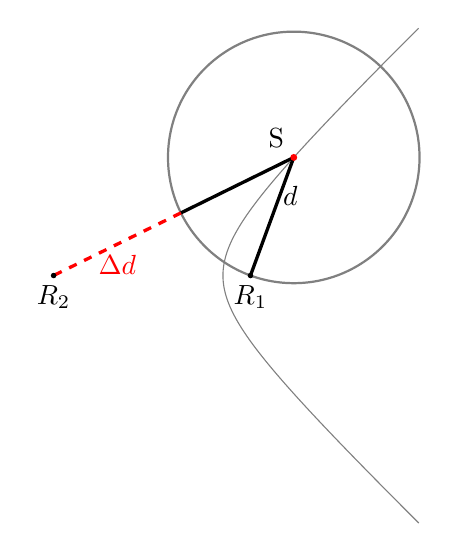
\begin{tikzpicture}[scale=0.5,>=Latex]
		
		%----------------------------------------
		% Receiver locations
		%----------------------------------------
		\coordinate (R1) at (2.5,0);
		\coordinate (R2) at (-2.5,0);
		
		%----------------------------------------
		% Source
		%----------------------------------------
		\coordinate (S) at (3.6,3.0);
		
		%----------------------------------------
		% Compute distances
		%----------------------------------------
		\path let \p1 = ($(R1)-(S)$) in
		\pgfextra{\xdef\radius{veclen(\x1,\y1)}};
		
		\path let \p1 = ($(R2)-(S)$) in
		\pgfextra{\xdef\distSRtwo{veclen(\x1,\y1)}};
		
		%----------------------------------------
		% Hyperbola locus
		% Shifted to align with receiver geometry
		%----------------------------------------
		% Receiver locations
		\coordinate (R1) at (2.5,0);
		\coordinate (R2) at (-2.5,0);
		
		% Source location
		\coordinate (S) at (3.6,3.0);
		
		
		%----------------------------------------
		% Compute hyperbola coefficients
		%----------------------------------------
		
		% c = half receiver spacing
		\pgfmathsetmacro{\cval}{2.5}
		
		% Distances from source to receivers
		\pgfmathsetmacro{\distOne}{sqrt((3.6-2.5)^2+(3.0)^2)}
		\pgfmathsetmacro{\distTwo}{sqrt((3.6+2.5)^2+(3.0)^2)}
		
		\pgfmathsetmacro{\aval}{abs(\distTwo-\distOne)/2}
		
		% b = sqrt(c^2-a^2)
		\pgfmathsetmacro{\bval}{sqrt(\cval*\cval-\aval*\aval)}
		
		% midpoint of receivers
		\pgfmathsetmacro{\xcenter}{(2.5+(-2.5))/2}
		
		% Right branch of hyperbola
		\draw[gray,thin,samples=200,smooth,domain=-2:2]
		plot ({\xcenter+\aval*cosh(\x)}, {\bval*sinh(\x)});
		
		%\node[blue] at (1.0,2.2) {Hyperbola};
		
		%----------------------------------------
		% Circle centered at source through R1
		%----------------------------------------
		\draw[gray,thick] (S) circle (\radius);
		
		%----------------------------------------
		% Point where S-R2 line intersects circle
		%----------------------------------------
		\pgfmathsetmacro{\ratio}{\radius/\distSRtwo}
		\coordinate (P) at ($(S)!\ratio!(R2)$);
		
		%----------------------------------------
		% Radius d to nearer receiver
		%----------------------------------------
		\draw[very thick]
		(S)--(R1)
		node[midway,above right] {$d$};
		
		%----------------------------------------
		% Same distance toward R2
		%----------------------------------------
		\draw[very thick]
		(S)--(P);
		
		%----------------------------------------
		% Excess path length
		%----------------------------------------
		\draw[very thick,dashed,red]
		(P)--(R2)
		node[midway,below] {$\Delta d$};
		
		%----------------------------------------
		% Points
		%----------------------------------------
		\fill (R1) circle (2pt);
		\fill (R2) circle (2pt);
		\fill[red] (S) circle (2.5pt);
		
		\node[below] at (R1) {$R_1$};
		\node[below] at (R2) {$R_2$};
		\node[above left] at (S) {S};
		
	\end{tikzpicture}
	\caption{Example TDOA Locus. $S$ is a source, $R$ is a receiver pair, and $\Delta d$ is the difference in arrival times expressed as an equivalent distance. The half hyperbola shows the set of possible source locations for a given $\Delta d$. }
	\end{figure}
\end{frame}

\begin{frame}{Where We Are Going}
	\begin{figure}
		\centering
		\includegraphics[width=1.0 \textwidth]{../../python_trilateration_sandbox/tdoa/loci_from_truth_points_2d.png}
		\caption{Pairwise receiver-emitter TDOA locus (2D)}
	\end{figure}
\end{frame}


\begin{frame}{Approach - Mock Chirp}
	We will be looking for this chirp in microphone recordings
	\begin{figure}
		\centering
%		\includegraphics[width=0.6 \textwidth]{../../python_correlation_sandbox/modern/saved_figs/06_example_sinct.pdf}
		\includegraphics[width=0.6 \textwidth]{../../python_correlation_sandbox/modern/saved_figs/10_realistic_sinct.pdf} 
		\caption{Asymptotically approaches 0 at $\pm \infty$}
	\end{figure}
\end{frame}

\begin{frame}{Approach - Mock Microphone Recording}
	Where precisely is the center of chirp in this audio sample?
	\begin{figure}
		\centering
		\includegraphics[width=0.68 \textwidth]{../../python_correlation_sandbox/modern/saved_figs/07_example_envt_sinct.pdf}
%		\includegraphics[width=0.68 \textwidth]{../../python_correlation_sandbox/modern/saved_figs/11_realistic_envt_sinct.pdf}
		\caption{Naive template matching in the time domain is inaccurate}
	\end{figure}
\end{frame}

\begin{frame}[fragile]{Approach - Cross Correlation}
	\begin{figure}
		
		Definition of Cross Correlation for complex signals with period $T$:
		\begin{align}
			(f \star g)(\tau) & = \int_{-\infty}^{+\infty} \overline{f(t)} g(t+\tau) \,dt = \int_{t_0}^{t_0+T} \overline{f(t)} g(t+\tau) \,dt
		\end{align}
		
	\end{figure}
	
	
	\begin{lstlisting}
int cross_correlation(vector sgnlA, vector sgnlB, int offset)
{
	int result = 0;
	for (int i = 0; i < sgnlA.size(); ++i)
	{
		size_t period = sgnlA.size();
		size_t indexB = (i+offset) % period; // pseudocode
		result += std::conj(sgnlA[i]) * sgnlB[indexB];
	}
	return result;
}
	\end{lstlisting}
\end{frame}


\begin{frame}{Cross Correlation}
	Cross-correlating the chirp with the input audio stream produces peaks where signals are "similar"
	\begin{figure}
		\centering
		\includegraphics[width=0.68 \textwidth]{../../python_correlation_sandbox/modern/saved_figs/08_example_correlation_surface_around_expected_peak_500_of_block_period.pdf}
		\caption{Results zoomed and centered around true peak location}
	\end{figure}
\end{frame}

\begin{frame}{Cross Correlation}
	True peak location will always be between 2 audio samples. 
	
	$\pm1$ sample  $\approx \pm 22.6 \mu$s.  range error $\approx \pm 0.3$in. angular error $ \approx \pm6.9^\circ$
	
	\begin{figure}
		\centering
		\includegraphics[width=0.7 \textwidth]{../../python_correlation_sandbox/modern/saved_figs/15_realistic_correlation_surface_around_expected_peak_10_of_block_period.pdf}
		\caption{Results zoomed and centered around true peak location}
	\end{figure}
\end{frame}


\begin{frame}{Solutions that don't work}
	\begin{figure}
		\begin{itemize}
			\item Interpolating the discrete correlation surface's derivative directly is inaccurate
			\item Fitting a 2nd order polynomial to the area around the raw audio is super inaccurate - unclean signal separation
			\item Fitting a 2nd order polynomial to the area around the correlation peak is also inaccurate - but worth investigating
		\end{itemize}
	\end{figure}
\end{frame}

\begin{frame}{Our Solution}
	\begin{figure}
		\begin{itemize}
			\item Re-express the chirp and recorded audio as continuous-time signals using the frequency domain
			\item Use those to express the correlation surface as a continuous-time function instead of a discrete-time one
			\item Find a coarse estimate of the peak using fast, industry standard algorithms (FFT)
			\item Refine the coarse estimate by using a root-solver on the analytic derivative of the continuous-time correlation surface
			\item Profittttt
		\end{itemize}
	\end{figure}
\end{frame}
	
\section{The Frequency Domain}

\begin{frame}{Simple Frequency Decomposition}
	\begin{figure}
		% Source - https://tex.stackexchange.com/q/127375
		% Posted by Shuhao Cao, modified by community. See post 'Timeline' for change history
		% Retrieved 2026-08-13, License - CC BY-SA 3.0
		
		$y(t) =  2.2 \sin(10t)  + \sin(22t )$
		
		\vspace{1.0cm}
		
		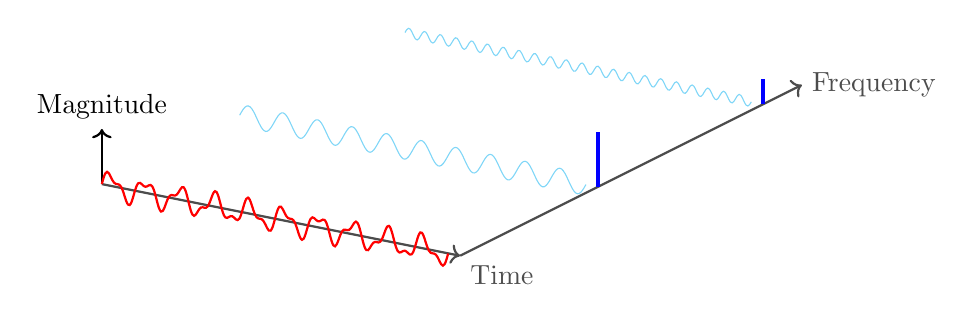
\begin{tikzpicture}[x={(1cm,0.5cm)},z={(0cm,0.5cm)},y={(1cm,-0.2cm)},scale=0.70]
			\draw[->,thick,black!70] (0,6.5,0) -- (6.2,6.5,0) node[right] {Frequency};
			\draw[->,thick,black!70] (0,0,0) -- (0,6.5,0) node[below right] {Time};
			\draw[->,thick] (0,0,0) -- (0,0,2) node[above] {Magnitude};
			\foreach \y in {2.5,5.5}{
				\draw [cyan!50, domain=0:2*pi,samples=200,smooth] 
				plot (\y,\x, {sin(4*\y*\x r)/\y });
				\draw[blue, ultra thick] (\y,6.5,0) -- (\y,6.5,5/\y);
			}
			\draw [red, thick, domain=0:2*pi,samples=200,smooth] 
			plot (0,\x, {0*sin(4*0.5*\x r)/0.5 + 0*sin(4*1.5*\x r)/1.5 + 1*sin(4*2.5*\x r)/2.5 + 0*sin(4*3.5*\x r)/3.5 + 0*sin(4*4.5*\x r)/4.5 + 1*sin(4*5.5*\x r)/5.5} );
		\end{tikzpicture}
		\caption{Simple signal represented in both time and frequency domains}
	\end{figure}
\end{frame}

\begin{frame}{Square Frequency Decomposition}
	\begin{figure}
		% Source - https://tex.stackexchange.com/q/127375
		% Posted by Shuhao Cao, modified by community. See post 'Timeline' for change history
		% Retrieved 2026-08-13, License - CC BY-SA 3.0
		
		\[
		y(t) =
		\frac{4}{\pi}
		\sum_{k=0}^{\infty}
		\frac{1}{2k+1}
		\sin\left((2k+1)\omega_0t\right)
		\]
		
		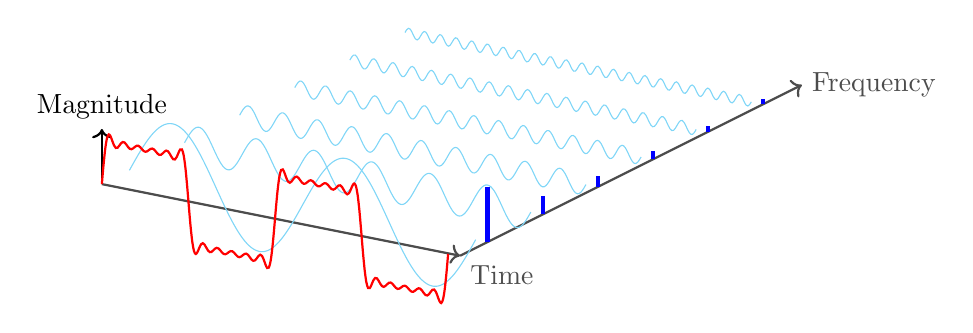
\begin{tikzpicture}[x={(1cm,0.5cm)},z={(0cm,0.5cm)},y={(1cm,-0.2cm)},scale=0.70]
			\draw[->,thick,black!70] (0,6.5,0) -- (6.2,6.5,0) node[right] {Frequency};
			\draw[->,thick,black!70] (0,0,0) -- (0,6.5,0) node[below right] {Time};
			\draw[->,thick] (0,0,0) -- (0,0,2) node[above] {Magnitude};
			\foreach \y in {0.5,1.5,...,5.5}{
				\draw [cyan!50, domain=0:2*pi,samples=200,smooth] 
				plot (\y,\x, {sin(4*\y*\x r)/\y });
				\draw[blue, ultra thick] (\y,6.5,0) -- (\y,6.5,1/\y);
			}
			\draw [red, thick, domain=0:2*pi,samples=200,smooth] 
			plot (0,\x, {sin(4*0.5*\x r)/0.5 + sin(4*1.5*\x r)/1.5 + sin(4*2.5*\x r)/2.5 + sin(4*3.5*\x r)/3.5 + sin(4*4.5*\x r)/4.5 + sin(4*5.5*\x r)/5.5} );
		\end{tikzpicture}
		\caption{Square wave signal represented in both time and frequency domains}
		\url{tex.stackexchange.com/q/127375}
		
	\end{figure}
\end{frame}

\begin{frame}{Euler Equation}
	\begin{figure}
		
		Any complex number can be represented as a complex exponential.
		\begin{align*}
			e^{i\omega t} = \cos(\omega t) + i\sin(\omega t)
		\end{align*}
		
		Multiplying complex numbers and complex exponentials together is like shifting the phase of a sine wave, especially when using conjugated weights and negative frequencies. More on this later...
		\begin{align*}
			(A+iB) e^{i\omega t} + (A-iB) e^{-i\omega t} &=2A \cos(\omega t) - 2B \sin(\omega t) \\ 
			&= C \cos(\omega t + \phi)  \\ 
		\end{align*}
	\end{figure}
\end{frame}

\begin{frame}{Discrete Fourier Transform}
	\begin{figure}
		\begin{align*}
		\mathbf{X} &= 	\mathcal{F}\{\mathbf{x}\} \\
		X[k] &= \sum_{n=0}^{N-1} x[n] e^{-i\frac{2\pi}{N}kn},
		\qquad k=0,1,\ldots,N-1 \\
		\begin{bmatrix}
			X[0]\\
			X[1]\\
			X[2]\\
			\vdots\\
			X[N-1]
		\end{bmatrix}
		&=
		\begin{bmatrix}
			1 & 1 & 1 & \cdots & 1\\
			1 & e^{-i\frac{2\pi}{N}} & e^{-i\frac{4\pi}{N}} & \cdots & e^{-i\frac{2\pi(N-1)}{N}}\\
			1 & e^{-i\frac{4\pi}{N}} & e^{-i\frac{8\pi}{N}} & \cdots & e^{-i\frac{4\pi(N-1)}{N}}\\
			\vdots & \vdots & \vdots & \ddots & \vdots\\
			1 & e^{-i\frac{2\pi(N-1)}{N}} &
			e^{-i\frac{4\pi(N-1)}{N}} &
			\cdots &
			e^{-i\frac{2\pi(N-1)^2}{N}}
		\end{bmatrix}
		\begin{bmatrix}
			x[0]\\
			x[1]\\
			x[2]\\
			\vdots\\
			x[N-1]
		\end{bmatrix} \\
		\mathbf{X} &= \mathbf{F}_N \mathbf{x}
		\end{align*}
	\end{figure}
\end{frame}

\begin{frame}{Example Chirp}
	\centering
	\begin{align*}
		sinc(t) &= \frac{sin(t)}{t} \\
		\mathcal{F}\{sinc(t)\} &= rect(\omega)
	\end{align*}
	\begin{columns}
		\begin{column}{0.48\textwidth}
			\centering
			\includegraphics[width=\linewidth]{../../python_correlation_sandbox/modern/saved_figs/00_sinct_10hz.pdf}
%			\captionof{figure}{$sinc(t)$}
		\end{column}
		\begin{column}{0.48\textwidth}
			\centering
			\includegraphics[width=\linewidth]{../../python_correlation_sandbox/modern/saved_figs/01_freq_mag_of_sinct_10hz.pdf}
%			\captionof{figure}{Second Caption}
		\end{column}
	\end{columns}
\end{frame}


\begin{frame}{Key Point - DFT Is A Matrix Multiplication}
		\begin{block}{Key Idea}
				The Discrete Time Fourier Transform (DFT) can be represented as a matrix multiplication.
			\end{block}
		
%		\vspace{0.3cm}
%		
%		\begin{alertblock}{Important}
%				The Discrete Time Fourier Transform (DFT) can be represented as a matrix multiplication.
%			\end{alertblock}
	\end{frame}
	
	
	
	\section{Solving for the Coarse Correlation Surface}
	
%\section{Naive Approach}

%\begin{frame}{Diagonal Equation Annotation}
%	
%	% Define an explanation node style
%	\tikzstyle{annot} = [font=\small, text=red, align=left]
%	
%	\begin{equation*}
%		% Mark a specific part of your equation using \tikzmarknode
%		\tikzmarknode{termA}{A} + B = C
%	\end{equation*}
%	
%	\begin{tikzpicture}[overlay, remember picture]
%		% Draw a diagonal arrow/line from the term to an offset coordinate and place text
%		\draw[->, thick, red] (termA.south west) -- ++(-0.5cm, -0.1cm) 
%		node[annot, below left] {Diagonal explanation text here};
%	\end{tikzpicture}
%	
%\end{frame}

\begin{frame}{Coarse Approach 1}
	\vspace{-0.5cm}
	\begin{align*}
		\begin{bNiceMatrix}
			x[0]\\
			x[1]\\
			x[2]\\
			\vdots
		\end{bNiceMatrix} &=
		\begin{bmatrix}
			1 & 1 & 1 & \cdots & 1\\
			1 & e^{i\frac{2\pi}{N}} & e^{i\frac{4\pi}{N}} & \cdots & e^{i\frac{2\pi(N-1)}{N}}\\
			1 & e^{i\frac{4\pi}{N}} & e^{i\frac{8\pi}{N}} & \cdots & e^{i\frac{4\pi(N-1)}{N}}\\
			\vdots & \vdots & \vdots & \ddots & \vdots\\
			1 & e^{i\frac{2\pi(N-1)}{N}} &
			e^{i\frac{4\pi(N-1)}{N}} &
			\cdots &
			e^{i\frac{2\pi(N-1)^2}{N}}
		\end{bmatrix}
		\begin{bNiceMatrix}
		X[0]\\
		X[1]\\
		X[2]\\
		\vdots\\
		X[N-1]
		\end{bNiceMatrix}
	\end{align*}
\end{frame}

\begin{frame}[fragile]{Coarse Approach 1}
	Compute correlation surface from $Nsamples=256$ complex coefficients. Live-compute twiddles. $O(n^2)$ complex multiplications
	
	\begin{lstlisting}[basicstyle=\ttfamily\scriptsize]
auto [coeffs_a_conj, coeffs_b] = // 256 coefficients each
array_r<Nsamples> surface;

auto time_start = time_func();
// loop is N*N = 256*256 = 65536 multiplications
for (size_t out_idx = 0; out_idx < Nsamples; ++out_idx)
{
	Real sum(0.0);
	for (size_t i = 0; i < coeffs_a_conj.size(); ++i)
	{
		auto a_conj = coeffs_a_conj[i];
		auto b = coeffs_b[i];
		
		Real freq = output_index * i / Real(domain::WindowSize);
		Complex term_i = a_conj * b * std::exp(twopi * freq);
		sum += term_i.real();
	}
	surface[out_idx] = sum;
}
auto time_stop = time_func();
	\end{lstlisting}
	
\end{frame}

\begin{frame}{Results}
	\coarsetable{1}{1}
\end{frame}


\begin{frame}{Coarse Approach 2}
	\vspace{-0.5cm}
	\begin{align*}
		\begin{bNiceMatrix}
			x[0]\\
			x[1]\\
			x[2]\\
			\vdots
		\end{bNiceMatrix} &=
		\begin{bNiceMatrix}
			\Block[fill=red!20]{9-1}{} 1 & 1 & \cdots & \Block[fill=red!20]{9-1}{} 1 & \Block[fill=yellow!20]{9-2}{} \cdots & 1\\
			1 & e^{i\frac{2\pi}{N}} & \cdots & -1 & \cdots & e^{i\frac{2\pi(N-1)}{N}}\\
			1 & e^{i\frac{4\pi}{N}} & \cdots & 1 & \cdots & e^{i\frac{4\pi(N-1)}{N}}\\
			\vdots & \vdots & \vdots & \vdots & \ddots & \vdots\\
			1 & e^{i\frac{2\pi(\frac{N}{2}-1)}{N}} & \cdots & -1 & \cdots & e^{i\frac{2\pi(\frac{N}{2}-1)(N-1)}{N}}\\
			1 & e^{i\frac{2\pi(\frac{N}{2})}{N}} & \cdots & 1 & \cdots &  e^{i\frac{2\pi(\frac{N}{2})(N-1)}{N}}\\
			1 & e^{i\frac{2\pi(\frac{N}{2}+1)}{N}} & \cdots & -1 & \cdots & e^{i\frac{2\pi(\frac{N}{2}+1)(N-1)}{N}}\\
			\vdots & \vdots & \vdots & \vdots & \ddots & \vdots\\
			1  &  e^{i\frac{2\pi(N-1)}{N}} &\cdots & -1 & \cdots & e^{i\frac{2\pi(N-1)^2}{N}}
		\end{bNiceMatrix}
		\begin{bNiceMatrix}
			\Block[fill=red!20]{1-1}{} \tikzmarknode{termDC}{X[0]}\\
			X[1]\\
			X[2]\\
			\vdots\\
			X[\frac{N}{2}-1] \\
			\Block[fill=red!20]{1-1}{} \tikzmarknode{termNY}{X[\frac{N}{2}]} \\
			\Block[fill=yellow!20]{3-1}{} X[\frac{N}{2}+1]\\
			\vdots \\
			\tikzmarknode{termNeg}{X[N-1]}
		\end{bNiceMatrix}
	\end{align*}
	
	
	\begin{tikzpicture}[overlay, remember picture]
		% Draw a diagonal arrow/line from the term to an offset coordinate and place text
		\draw[<-, thick, red] (termDC.west) -- ++(-0.5cm, 1.26cm) 
		node[annot, left] {DC Coefficient (freq=0 or +N or -N)};
	\end{tikzpicture}
	
	\begin{tikzpicture}[overlay, remember picture]
		% Draw a diagonal arrow/line from the term to an offset coordinate and place text
		\draw[<-, thick, red] (termNY.west) -- ++(-1.0cm, 3.5cm) 
		node[annot, left] {Nyquist Coefficient (freq=+N/2 or -N/2)};
	\end{tikzpicture}
	
	\begin{tikzpicture}[overlay, remember picture]
		% Draw a diagonal arrow/line from the term to an offset coordinate and place text
		\draw[<-, thick, red] (termNeg.south) -- ++(-0.1cm, -1.0cm) 
		node[annot, left] {Coefficients for negative freqs. complex conjugates of the positive freqs};
	\end{tikzpicture}
\end{frame}

\begin{frame}[fragile]{Coarse Approach 2}
	Exploit conjugate symmetry to compute correlation surface using $\frac{Nsamples}{2}+1=129$ complex coefficients . Live-compute twiddles. $O(n^2)$ complex multiplications. Multiply the terms with conjugate symmetry by 2 and take their real component since $z + \bar{z} = 2\operatorname{Re}(z) $
	
	
	\begin{lstlisting}[basicstyle=\ttfamily\scriptsize]
auto [coeffs_a_conj, coeffs_b] = // 129 coefficients each
array_r<Nsamples> surface;
		
for (size_t i=1; i < coeffs_a_conj.size()-1; ++i)
{
	coeffs_a_conj[i] *= 2;
}
		
auto time_start = time_func();
// same nested loop structure. 
// Now N*(N/2+1) = 256*129 = 33024 mults
auto time_stop = time_func();
	\end{lstlisting}
	
\end{frame}


\begin{frame}{Results}
	\coarsetable{1}{2}
\end{frame}


\begin{frame}{Coarse Approach 3}
	\vspace{-0.5cm}
	\begin{align*}
		\begin{bNiceMatrix}
			x[0]\\
			x[1]\\
			x[2]\\
			\vdots
		\end{bNiceMatrix} &=
		\begin{bNiceMatrix}
			1 & 2 & 2 & \Block[fill=red!20]{9-1}{} \cancel{\cdots} & 1 & \cancel{\cdots} \\
			1 & 2e^{i\frac{2\pi}{N}} & 2e^{i\frac{4\pi}{N}} & \cancel{\cdots} & -1 & \cancel{\cdots} \\
			1 & 2e^{i\frac{4\pi}{N}} & 2e^{i\frac{8\pi}{N}} & \cancel{\cdots} & 1 & \cancel{\cdots} \\
			\vdots & \vdots & \vdots & \vdots & \ddots & \vdots\\
			1 & 2e^{i\frac{2\pi(\frac{N}{2}-1)}{N}} & 2e^{i\frac{4\pi(\frac{N}{2}-1)}{N}} & \cancel{\cdots} & -1 & \cancel{\cdots} \\
			1 & 2e^{i\frac{2\pi(\frac{N}{2})}{N}} & 2e^{i\frac{4\pi(\frac{N}{2})}{N}} & \cancel{\cdots} & 1 & \cancel{\cdots} \\
			1 & 2e^{i\frac{2\pi(\frac{N}{2}+1)}{N}}  & 2e^{i\frac{4\pi(\frac{N}{2}+1)}{N}}& \cancel{\cdots} & -1 & \cancel{\cdots} \\
			\vdots & \vdots & \vdots & \vdots & \vdots & \ddots \\
			1  &  2e^{i\frac{2\pi(N-1)}{N}} & 2e^{i\frac{4\pi(N-1)}{N}} & \cancel{\cdots} & -1 & \cancel{\cdots} 
		\end{bNiceMatrix}
		\begin{bNiceMatrix}
			X[0]\\
			X[1]\\
			X[2]\\
			\Block[fill=red!20]{1-1}{} \tikzmarknode{termsNearZero}{\vdots}\\
			X[\frac{N}{2}] \\
			\tikzmarknode{termNeg}{\vdots}
		\end{bNiceMatrix}
	\end{align*}
	
	
	
	\begin{tikzpicture}[overlay, remember picture]
		% Draw a diagonal arrow/line from the term to an offset coordinate and place text
		\draw[<-, thick, red] (termsNearZero.north west) -- ++(-1.0cm, 3.0cm) 
		node[annot, left] {Most coefficients $\approx 0$ from chirp)};
	\end{tikzpicture}
\end{frame}


\begin{frame}[fragile]{Coarse Approach 3}
	Compute correlation surface using $N=60$ complex coefficients by omitting coefficients near $0$ and exploiting conjugate symmetry. Live compute twiddles. $O(nm)$
	
	\begin{lstlisting}[basicstyle=\ttfamily\scriptsize]
auto [coeffs_a_conj, coeffs_b] = // 129 coefficients each
array_r<Nsamples> surface;

for (size_t i=1; i < coeffs_a_conj.size()-1; ++i)
{
	coeffs_a_conj[i] *= 2;
}

// count the first M terms with magnitude larger than a threshold

auto time_start = time_func();
// same nested loop structure. Now N*M = 256*60 = 15360 mults
auto time_stop = time_func();
	\end{lstlisting}
	
\end{frame}

\begin{frame}{Approach 3 Not Viable}
	\begin{itemize}
		\item The terms that were near zero were not identically zero. 
		\item This introduced an error of $\approx$ 0.1 on a scale of 1E3 - 1E4)
		\item Previous errors were \textless 1E-3
	\end{itemize}
\end{frame}

\begin{frame}{Results}
	\coarsetable{1}{3}
\end{frame}


\begin{frame}[fragile]{Coarse Approach 4}
	Compute correlation surface using $Nsamples=256$ complex coefficients by exploiting conjugate symmetry. precompute twiddles. $O(n^2)$
	
	\begin{lstlisting}[basicstyle=\ttfamily\scriptsize, 
		linebackgroundcolor={%
			\ifnum\value{lstnumber}=10 \color{yellow!30}\fi
		}]
auto time_start = time_func();

constexpr size_t Noutputs_used = Nsamples/2;
for (size_t out_idx = 0; out_idx < Noutputs_used; ++out_idx)
{
	Real sum(0.0);
	for (size_t i = 0; i < Ncoeffs; ++i)
	{
		auto b = coeffs_b[i];
		Complex term_i =  b * Wn[out_idx][i]; // a_conj baked in
		sum += term_i.real();
	}
	surface[out_idx] = sum;
}
auto time_stop = time_func();
	\end{lstlisting}
	
\end{frame}


\begin{frame}{Results}
	\coarsetable{1}{4}
\end{frame}


\begin{frame}[fragile]{Coarse Approach 5}
	A Fourier Transform can be computed recursively. This is Radix-2:
	
	\begin{align}
		\mathbf{X} &= \mathcal{F}\{\mathbf{x}\}  \\
		X[k] &= \sum_{n=0}^{N-1} x[n] e^{-i\frac{2\pi}{N}kn}, \qquad k=0,1,\ldots,N-1 \\
		&= \sum_{n=0}^{N/2-1} x[n] e^{-i\frac{2\pi}{N}k(2n)} + \sum_{n=0}^{N/2-1} x[n] e^{-i\frac{2\pi}{N}k(2n+1)} \\
		&= \sum_{n=0}^{N/2-1} x[n] e^{-i\frac{2\pi}{N/2}kn} + e^{-i\frac{2\pi}{N}kn} \sum_{n=0}^{N/2-1} x[n] e^{-i\frac{2\pi}{N/2}kn} \\
		X[k] &= \mathcal{F}\{\mathbf{x}_{\texttt{evens}}\}  + e^{-i\frac{2\pi}{N}kn} \mathcal{F}\{\mathbf{x}_{\texttt{odds}}\} \\
		X[k+\frac{N}{2}] &= \mathcal{F}\{\mathbf{x}_{\texttt{evens}}\}  - e^{-i\frac{2\pi}{N}kn} \mathcal{F}\{\mathbf{x}_{\texttt{odds}}\}
	\end{align}
	turtles all the way down
	
\end{frame}

\begin{frame}
	\begin{itemize}
		\item You can radix by any prime number, but N must be a multiple/power of that number
		\item Radix-2, Radix-3, Radix-4 most common
		\item Each radix level trades fewer multiplications for code complexity and cache performance
		\item Modern FFT libraries are extremely complicated and performance is very hardware dependent 
		\item Not discussed here: in place? bit reversal for high-radix?
		\item Not discussed here: decimation in time / decimation in frequency
	\end{itemize}
\end{frame}

\begin{frame}[fragile]{Coarse Approach 5}
	
	\begin{lstlisting}[basicstyle=\ttfamily\scriptsize]
// N*log2(N) = 256*8 = 2048
void butterfly_dit(Complex* buffer) {
	// en.wikipedia.org/wiki/Cooley%E2%80%93Tukey_FFT_algorithm
	size_t m = 1;
	size_t exp_stride = Nsamples;
	for (size_t s = 1; s <= n_bits; ++s) {
		size_t mHalf = m;
		m *= 2;
		for (size_t k = 0; k < Nsamples; k+= m) {
			for (size_t j = 0; j < mHalf; ++j) {
				auto omega = twiddles[exp_stride*j];
				size_t indA = k + j;
				size_t indB = indA + mHalf;
				auto u = buffer[indA];
				auto t = omega * buffer[indB];
				buffer[indA] = u + t;
				buffer[indB] = u - t;
			}
		}
		exp_stride /= 2;
	}
}
	\end{lstlisting}
	
\end{frame}


\begin{frame}{Results}
	\coarsetable{1}{5}
\end{frame}


\begin{frame}
	Oh wait, computing twiddles with \texttt{std::exp} is less efficient and less accurate than \texttt{std::polar} since \texttt{std::exp} is generalized for complex powers and contains branches. cppreference says \texttt{std::polar} is ~4.5 times faster: https://en.cppreference.com/cpp/numeric/complex/polar
\end{frame}

\begin{frame}
\coarsetable{2}{5}
\end{frame}

\begin{frame}
	% performance on Teensy	
	\coarsetable{5}{5}
\end{frame}



	\section{Refining the Coarse Solution}
	
%\section{Naive Approach}


\begin{frame}{Refinement}
	True peak location will always be between 2 audio samples. 
	\begin{figure}
		\centering
		\includegraphics[width=0.7 \textwidth]{../../python_correlation_sandbox/modern/saved_figs/15_realistic_correlation_surface_around_expected_peak_10_of_block_period.pdf}
		\caption{Results zoomed and centered around true peak location}
	\end{figure}
\end{frame}

\begin{frame}{Refinement}
	\begin{align}
		(y_1 \star y_2) (\tau) & = T \sum_{m = -N/2}^{N/2-1} \overline{A_m} B_{m} \exp{(\twopii f_m \tau)}
	\end{align}
	\vspace{0.5cm}
	\begin{align}
		\diff{^{(n)}}{\tau^{(n)}} (y_1 \star y_2)(\tau) & = (\twopii)^{n} T \sum_{m = -N/2}^{N/2-1} f_m^n \overline{A_m} B_m \exp{(\twopii f_m \tau)} \\
		&\text{where $f^n_{-N/2} = 0$ for odd n}
	\end{align}
\end{frame}


%\begin{frame}{xxxxxxx}
%	\begin{figure}
%		\centering
%		\includegraphics[width=0.7 \textwidth]{../../python_correlation_sandbox/modern/saved_figs/12_realistic_correlation_surface_around_expected_peak_500_of_block_period.pdf}
%		\caption{Correlation surface}
%	\end{figure}
%\end{frame}


\begin{frame}{Correlation Surface Derivatives}
	The correlation peak can be found from the zero-crossing of the first derivative. Let's put it in a root solver and let it run a couple iterations. 
	
	
	\centering
%	\begin{align*}
%		sinc(t) &= \frac{sin(t)}{t} \\
%		\mathcal{F}\{sinc(t)\} &= rect(\omega)
%	\end{align*}
	\begin{columns}
		\begin{column}{0.5\textwidth}
			\centering
			\includegraphics[width=\linewidth]{../../python_correlation_sandbox/modern/saved_figs/15_realistic_correlation_surface_around_expected_peak_10_of_block_period.pdf}
			%			\captionof{figure}{$sinc(t)$}
		\end{column}
		\begin{column}{0.5\textwidth}
			\centering
			\includegraphics[width=\linewidth]{../../python_correlation_sandbox/modern/saved_figs/16_realistic_fracddtau_correlation_surface_around_expected_peak_10_of_block_period.pdf}
			%			\captionof{figure}{Second Caption}
		\end{column}
	\end{columns}
\end{frame}


\begin{frame}[fragile]{Newton Solver}
	Solving for the corr peak requires evaling the 0th, 1st, and 2nd derivatives
		\begin{align}
			x_{i+1} \leftarrow x_i - \frac{f'(x_i)}{f''(x_i)}
		\end{align}
	
	
	\begin{lstlisting}[basicstyle=\ttfamily\scriptsize, 
		linebackgroundcolor={%
			\ifnum\value{lstnumber}=9 \color{yellow!30}\fi
			\ifnum\value{lstnumber}=10 \color{yellow!30}\fi
			\ifnum\value{lstnumber}=11\color{yellow!30}\fi
		}]
struct NewtonSolver
{
	template <typename CallableT>
	static Solution solve(const CallableT &fd0_fd1_fd2, Precision guess_tau_s, size_t n_steps = 4)
	{
		Precision x_n = guess_tau_s;
		for (size_t i = 0; i < n_steps; ++i)
		{
			auto [f_d0, f_d1, f_d2] = fd0_fd1_fd2(x_n);
			auto update = f_d1 / f_d2;
			x_n = x_n - update;
		}
		
		auto [f_d0, f_d1, f_d2] = fd0_fd1_fd2(x_n);
		return Solution{.x_final=x_n, .f_at_x_final=f_d0};
	}
};
	\end{lstlisting}
\end{frame}

\begin{frame}{The Refinement Problem}
	\vspace{-0.5cm}
	Fundamentally different problem now since we need only data point, but at a completely arbitrary location
	\begin{align*}
		\begin{bNiceMatrix}
			\\
			\\
			x[12.34]\\
			\\
			\\
		\end{bNiceMatrix} &=
		\begin{bmatrix}
			&  &  &  & \\
			&  &  &  & \\
			1 & e^{i\frac{2\pi(12.34)}{N}} & e^{i\frac{4\pi(12.34)}{N}} & \cdots & e^{i\frac{2\pi(12.34)(N-1)}{N}}\\
			 &  &  &  & \\
			 & & & & \\
			 & & & & % \\
		\end{bmatrix}
		\begin{bNiceMatrix}
			X[0]\\
			X[1]\\
			X[2]\\
			\vdots\\
			X[N-1]
		\end{bNiceMatrix}
	\end{align*}
\end{frame}


\begin{frame}{Refinement Approach 1}
	\begin{itemize}
		\item One function to compute the function at any derivative order
		\item Evaluate multiple derivatives simultaneously via template metaprogramming
		\item Compiler cannot optimize or reuse calls to std::exp or std::polar
	\end{itemize}
\end{frame}

\begin{frame}[fragile]{Refinement Approach 1}
	\begin{lstlisting}[basicstyle=\ttfamily\scriptsize, 
		linebackgroundcolor={%
			\ifnum\value{lstnumber}=1 \color{yellow!30}\fi
			\ifnum\value{lstnumber}=7 \color{yellow!30}\fi
			\ifnum\value{lstnumber}=8 \color{yellow!30}\fi
			\ifnum\value{lstnumber}=24 \color{yellow!30}\fi
		}]
template <size_t deriv_order, typename TauT>
auto correlate_impl(const CoeffsT &B, const TauT tau) const
{
	Real sum(0.0);
	for (size_t i = 0; i < Ncoeffs; ++i)
	{
		auto Wn = std::polar(1, constants::twopi * freqs[i] * tau);
		Complex term_i = coeffs_a_conj_and_f[deriv_order][i]*B[i]*Wn;
		
		// pull only the real/imag parts. components not taken are 0
		if constexpr(deriv_order%4==0)      sum+=term_i.real();
		else if constexpr(deriv_order%4==1) sum-=term_i.imag();
		else if constexpr(deriv_order%4==2) sum-=term_i.real();
		else if constexpr(deriv_order%4==3) sum+=term_i.imag();
	}
	return sum;
}
	\end{lstlisting}
	
\end{frame}


\begin{frame}[fragile]{Refinement Approach 1}
	\begin{lstlisting}[basicstyle=\ttfamily\scriptsize, 
		linebackgroundcolor={%
			\ifnum\value{lstnumber}=6 \color{yellow!30}\fi
			\ifnum\value{lstnumber}=14 \color{yellow!30}\fi
		}]
template <typename TauT, size_t... indicesT>
auto correlate_and_derive_impl(const CoeffsT &B, const TauT tau, std::integer_sequence<size_t, indicesT...>) const
{
	using correlation_type = decltype(correlate_impl<0>(B, tau));
	std::array<correlation_type, sizeof...(indicesT)> ret;
	((ret[indicesT] = correlate_impl<indicesT>(B, tau)), ...);
	return ret;
}


template <size_t deriv_order, typename TauT = Real>
auto correlate_and_derive_v0(const CoeffsT &B, const TauT tau) const
{
	return correlate_and_derive_impl(B, tau, std::make_index_sequence<deriv_order + 1>());
}
	\end{lstlisting}
	
\end{frame}

\begin{frame}{Results}
	\refinementtable{3}{1}
\end{frame}


\begin{frame}{Refinement Approach 2}
	\begin{itemize}
		\item Compute all derivative orders in the same function
		\item Evaluate all twiddles on each iteration
	\end{itemize}
\end{frame}

\begin{frame}[fragile]{Refinement Approach 2}
	\begin{lstlisting}[basicstyle=\ttfamily\scriptsize, 
		linebackgroundcolor={%
			\ifnum\value{lstnumber}=8 \color{yellow!30}\fi
			\ifnum\value{lstnumber}=9 \color{yellow!30}\fi
			\ifnum\value{lstnumber}=13 \color{yellow!30}\fi
		}]
template <size_t deriv_order, typename TauT = Real>
auto correlate_and_derive_v1(const CoeffsT &B, const TauT tau) {
	constexpr size_t Norders = deriv_order + 1; // include orig fcn
	
	std::array<Real, Norders> sum; // fill 0
	for (size_t i = 0; i < Ncoeffs; ++i)
	{
		auto Wn = std::polar(1, twopi * freqs[i] * tau);
		auto coeff_b_and_Wn = B[i] * Wn;
		
		for (size_t order = 0; order < Norders; ++order)
		{
			Complex term_i=coeffs_a_conj_and_f[order][i]*coeff_b_and_Wn;
			
			// pull only the real/imag parts. components not taken are 0
			if constexpr(derivative_order%4==0)      sum+=term_i.real();
			else if constexpr(derivative_order%4==1) sum-=term_i.imag();
			else if constexpr(derivative_order%4==2) sum-=term_i.real();
			else if constexpr(derivative_order%4==3) sum+=term_i.imag();
		}
	} return sum;
}
	\end{lstlisting}
	
\end{frame}


\begin{frame}{Results}
	\refinementtable{3}{2}
\end{frame}


\begin{frame}{Discrete Fourier Transform (Summation Form)}
	\begin{align}
		x[k] &= \sum_{n=0}^{N-1} X[n] e^{i\frac{2\pi}{N}kn}, \qquad k=0,1,\ldots,N-1
	\end{align}
	\vspace{0.5cm}
	\begin{align}
	\tikzmarknode{precompute}{W} &= e^{i\frac{2\pi}{N}\tau} \\
	x(k) &= \sum_{n=0}^{N-1} X[n] \tikzmarknode{update}{W^n}, \qquad k=0,1,\ldots,N-1
	\end{align}
	
	\begin{tikzpicture}[overlay, remember picture]
		% Draw a diagonal arrow/line from the term to an offset coordinate and place text
		\draw[<-, thick, red] (precompute.west) -- ++(-1.0cm, 0.5cm) 
		node[annot, above] {Precompute once};
	\end{tikzpicture}
	
	\begin{tikzpicture}[overlay, remember picture]
	% Draw a diagonal arrow/line from the term to an offset coordinate and place text
	\draw[<-, thick, red] (update.south) -- ++(0.5cm, -1.0cm) 
	node[annot, below] {Update iteratively since $W^n = W^{n-1} \ W$};
	\end{tikzpicture}
\end{frame}

\begin{frame}{Refinement Approach 3}
	\begin{itemize}
		\item Compute all derivatives in the same function
		\item Evaluate one twiddle. Use it to recursively compute the rest
		\item Potential accuracy hit for some scenarios 
	\end{itemize}
\end{frame}


\begin{frame}[fragile]{Refinement Approach 3}
	\begin{lstlisting}[basicstyle=\ttfamily\scriptsize, 
		linebackgroundcolor={%
			\ifnum\value{lstnumber}=5 \color{yellow!30}\fi
			\ifnum\value{lstnumber}=6 \color{yellow!30}\fi
			\ifnum\value{lstnumber}=15 \color{yellow!30}\fi
			\ifnum\value{lstnumber}=22 \color{yellow!30}\fi
		}]
template <size_t deriv_order, typename TauT = Real>
auto correlate_and_derive_v2(const CoeffsT &B, const TauT tau) {
	constexpr size_t Norders = deriv_order + 1; // include orig fcn
	
	Complex Wn(1,0);
	Complex W1 = std::polar(1, twopi * freqs[1] * tau);
	
	std::array<Real, Norders> sum; // fill 0
	for (size_t i = 0; i < Ncoeffs; ++i)
	{
		auto coeff_b_and_Wn = B[i] * Wn;
		
		for (size_t order = 0; order < Norders; ++order)
		{
			Complex term_i=coeffs_a_conj_and_f[order][i]*coeff_b_and_Wn;
			
			if (order % 4 == 0)          sum[order] += term_i.real();
			else if (order % 4 == 1)     sum[order] -= term_i.imag();
			else if (order % 4 == 2)     sum[order] -= term_i.real();
			else /*if (order % 4 == 3)*/ sum[order] += term_i.imag();
		}
		Wn *= W1;
	} return sum;
}
	\end{lstlisting}
	
\end{frame}


\begin{frame}{Results}
	\refinementtable{3}{3}
\end{frame}





	
\section{Hardware Implementation}

%\section{Naive Approach}


\begin{frame}%{Linear Arrangement}
	\begin{figure}
		\centering
		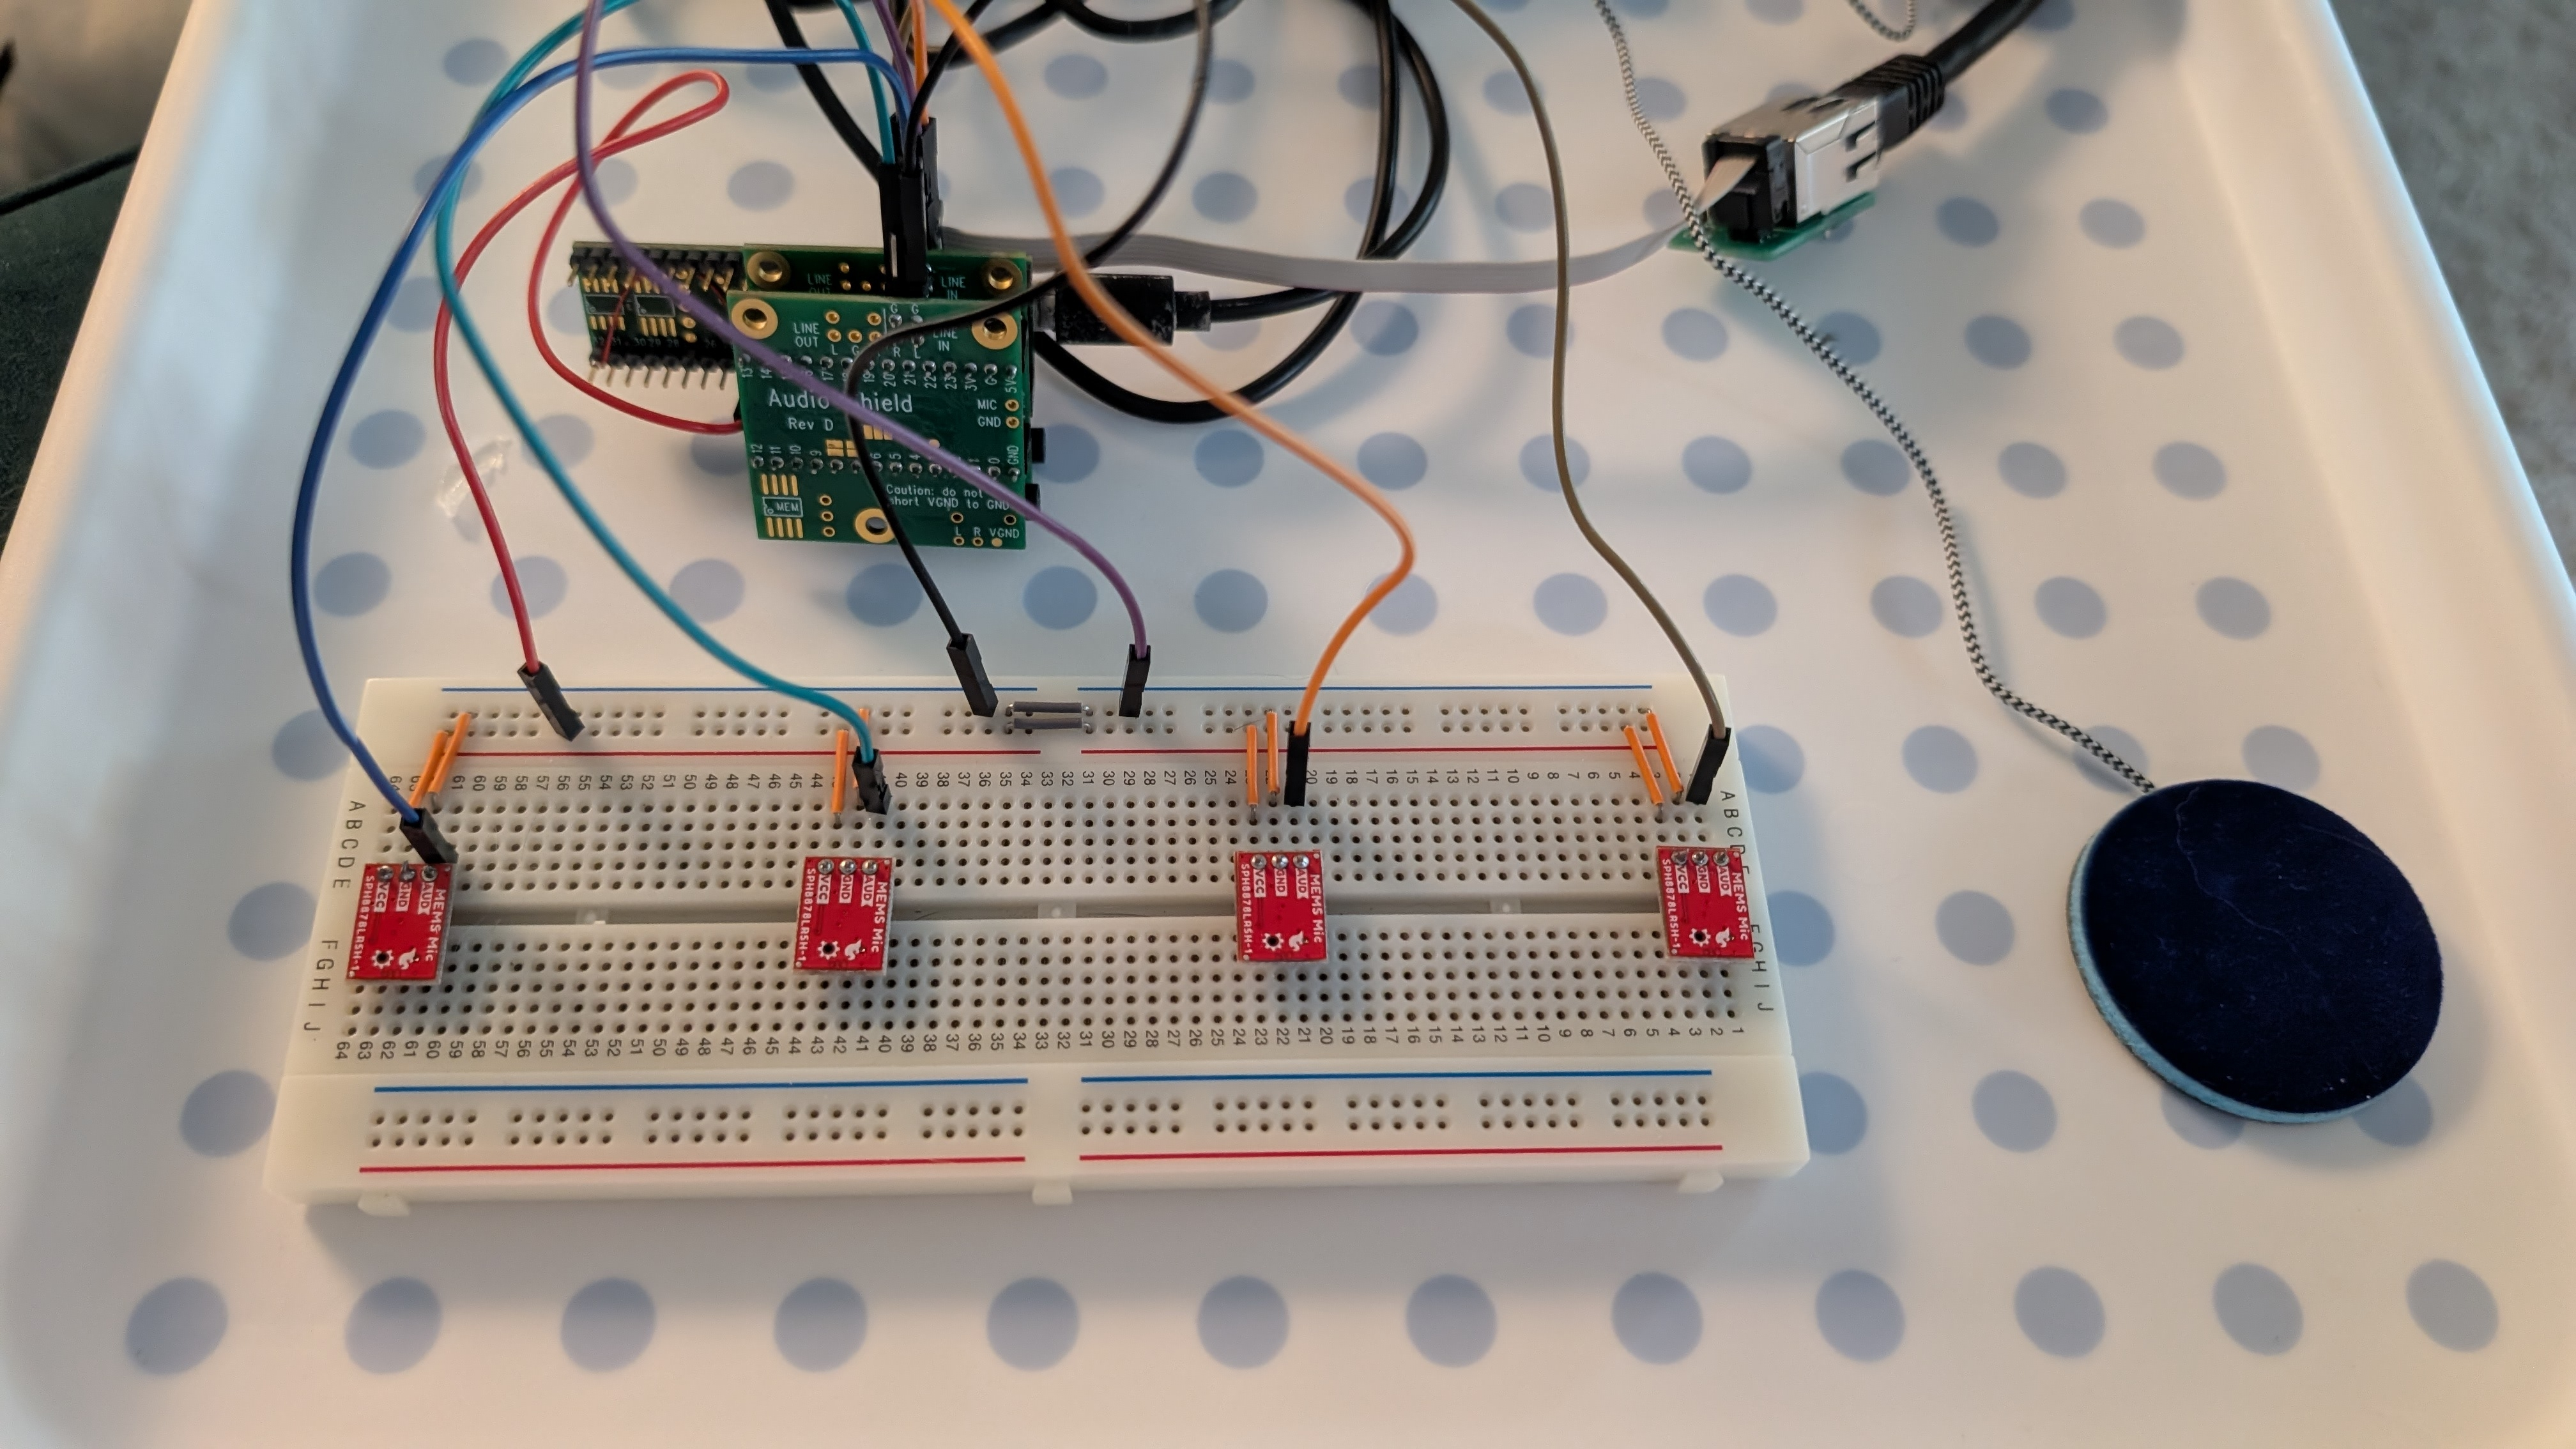
\includegraphics[width=0.95 \textwidth]{figures/hardware_01.jpeg}
		\caption{Left: Sparkfun analog MEMS microphones. Right: Speaker}
	\end{figure}
\end{frame}

\begin{frame}{Hardware Implementation - Phase Check}
	\begin{itemize}
		\item Connect all 4 analog microphone input wires to the same microphone condenser unit
		\item Good way to confirm that all 4 analog audio channels are phase locked
		\item This is not a "given" for many circuits. There are many places an audio board can introduce (non-deterministic) lag
	\end{itemize}
\end{frame}

\begin{frame}%{Phase Check}
	\begin{figure}
		\centering
		\includegraphics[width=0.95 \textwidth]{figures/recording_phase_check_02.png}
		\caption{Phase Check - all 4 analog inputs sampling the same mic}
	\end{figure}
\end{frame}

\begin{frame}%{Phase Check}
	\begin{figure}
		\centering
		\includegraphics[width=0.95 \textwidth]{figures/recording_phase_check_01.png}
		\caption{Phase Check - all 4 analog inputs sampling the same mic}
	\end{figure}
\end{frame}


\begin{frame}{Hardware Implementation - Linear Distance Measurement}
	\begin{itemize}
		\item Arrange all 4 mics in a straight line with known distances (50.4mm) between them
		\item We should be able to measure the distance between the mics using our algorithms*
	\end{itemize}
\end{frame}

\begin{frame}%{Linear Arrangement}
	\begin{figure}
		\centering
		\includegraphics[width=0.95 \textwidth]{figures/recording_linear_arrangement_03.png}
		\caption{Linear Arrangement - all mics in a line}
	\end{figure}
\end{frame}

\begin{frame}%{Linear Arrangement}
	\begin{figure}
		\centering
		\includegraphics[width=0.95 \textwidth]{figures/recording_linear_arrangement_02.png}
		\caption{Linear Arrangement - all mics in a line}
	\end{figure}
\end{frame}


\begin{frame}%{Linear Arrangement}
	\begin{figure}
		\centering
		\includegraphics[width=0.95 \textwidth]{figures/recording_linear_arrangement_01.png}
		\caption{Linear Arrangement - all mics in a line}
	\end{figure}
\end{frame}


%channels 0&1: mic[0].time_idx: 20985245-0.02[], mic[1].time_idx: 20985240-0.89[], TDOA: 133.07us, linear_intra_mic_distance: 45.64mm
%channels1&2: mic[1].time_idx: 20985240-0.89[], mic[2].time_idx: 20985233-0.78[], TDOA: 156.21us, linear_intra_mic_distance: 53.58mm
%channels 2&3: mic[2].time_idx: 20985233-0.78[], mic[3].time_idx: 20985225-0.13[], TDOA: 166.68us, linear_intra_mic_distance: 57.17mm
%channels 0&2: mic[0].time_idx: 20985245-0.02[], mic[2].time_idx: 20985233-0.78[], TDOA: 289.28us, linear_intra_mic_distance: 99.22mm
%channels 0&3: mic[0].time_idx: 20985245-0.02[], mic[3].time_idx: 20985225-0.13[], TDOA: 455.96us, linear_intra_mic_distance: 156.39mm
%channels 1&3: mic[1].time_idx: 20985240-0.89[], mic[3].time_idx: 20985225-0.13[], TDOA: 322.89us, linear_intra_mic_distance: 110.75mm
%
%
%chirp detected between channels 0&1: mic[0].time_idx: 3048808-0.57[], mic[1].time_idx: 3048814-0.06[], TDOA: -147.46us, linear_intra_mic_distance: -50.58mm
%chirp detected between channels 0&2: mic[0].time_idx: 3048808-0.57[], mic[2].time_idx: 3048821-0.63[], TDOA: -293.38us, linear_intra_mic_distance: -100.63mm
%chirp detected between channels 0&3: mic[0].time_idx: 3048808-0.57[], mic[3].time_idx: 3048827-0.51[], TDOA: -432.10us, linear_intra_mic_distance: -148.21mm
%chirp detected between channels 1&2: mic[1].time_idx: 3048814-0.06[], mic[2].time_idx: 3048821-0.63[], TDOA: -145.91us, linear_intra_mic_distance: -50.05mm
%chirp detected between channels 1&3: mic[1].time_idx: 3048814-0.06[], mic[3].time_idx: 3048827-0.51[], TDOA: -284.64us, linear_intra_mic_distance: -97.63mm
%chirp detected between channels 2&3: mic[2].time_idx: 3048821-0.63[], mic[3].time_idx: 3048827-0.51[], TDOA: -138.72us, linear_intra_mic_distance: -47.58mm
\begin{frame}[fragile]{Linear Distance Measurement}
	
	\begin{figure}
		\centering
		\[
		\begin{array}{c c|cccc}
			& & \multicolumn{4}{c}{\mathbf{B}} \\
			& & \multicolumn{4}{c}{\rule{0pt}{0.5em}} \\[-1em]
			& & ch0 & ch1 & ch2 & \cellcolor{red!20}ch3 \\ \hline
			& ch0 &       & 50.58  & 100.63 & \cellcolor{red!20}148.21 \\
			\mathbf{A} & ch1 &       &        & 50.05  & \cellcolor{red!20}97.63  \\
			& ch2 &       &        &         & \cellcolor{red!20}47.58
		\end{array}
		\]
		
		
		
		
		
		\caption{$\Delta t$ between channels A and B}
	\end{figure}
	
	\vspace{-0.5em}
	
	\begin{itemize}
		\item Runtime: $\approx 222\,\mu\mathrm{s}$ per channel
		\item Total runtime  $< 1\,\mathrm{ms}$ for all 4 channels
		\item 8-channel audio lets gooooo
	\end{itemize}
	
\end{frame}







	
	\section{Misc}
	
	\begin{frame}{Unclean Frequency Separation}
		\begin{figure}
			\centering
			\includegraphics[width=0.7 \textwidth]{../../python_correlation_sandbox/modern/saved_figs/09_example_correlation_surface_around_expected_peak_10_of_block_period.pdf}
			\caption{Correlation surface for unclean frequency seperation}
		\end{figure}
	\end{frame}
	
	\begin{frame}{Clean Frequency Seperation}
		\begin{figure}
			\centering
			\includegraphics[width=0.7 \textwidth]{../../python_correlation_sandbox/modern/saved_figs/18_realistic_frequency_coefficient_magnitude.pdf}
			\caption{Clean separation in frequency domain}
		\end{figure}
	\end{frame}
	
	\begin{frame}{Improvements}
		\begin{itemize}
			\item Investigate fitting a second order polynomial to the correlation surface and analytically finding its peak location
			\item Investigate just after around chirp peak in recordings
			\item 8-channel (multiple Teensy's?)
			\item PDM microphones for higher quality inputs and phase correction
			\end{itemize}
	\end{frame}

	
	
%	
\begin{frame}{Mathematical Formulation}
	
	\[
	f(x)=\sum_{i=1}^{n}x_i^2
	\] 
	
	\[
	\frac{dy}{dx}=2x
	\]
	
\end{frame}
%	\begin{frame}[fragile]{Example C++ Code}
	
	\begin{lstlisting}
#include <iostream>

int main()
{
	std::cout << "Hello World" << std::endl;
	
	return 0;
}
	\end{lstlisting}
	
\end{frame}
%	
\begin{frame}{Example Figure}
	
%	\begin{figure}
%		\centering
%		\includegraphics[width=0.7\textwidth]{figures/results_10.pdf}
%		\caption{Example caption}
%	\end{figure}
	
\end{frame}
%	
\begin{frame}{Example Table}
	
	\centering
	
	\begin{tabular}{lcc}
		\toprule
		Method & Accuracy & Time \\
		\midrule
		Method A & 95\% & 2.1 s \\
		Method B & 97\% & 1.8 s \\
		Method C & 99\% & 1.2 s \\
		\bottomrule
	\end{tabular}
	
\end{frame}
%    
\begin{frame}{Discussion}
	
	\begin{itemize}
		\item Interpretation of results
		\item Strengths
		\item Limitations
		\item Future work
	\end{itemize}
	
\end{frame}	
%    
\begin{frame}{Takeaways}
	
	\begin{block}{Summary}
		\begin{itemize}
			\item Main finding
			\item Key contribution
			\item Future directions
		\end{itemize}
	\end{block}
	
\end{frame}
	
	
	%------------------------------------------------
	% References
	%------------------------------------------------
	
%	\begin{frame}[allowframebreaks]{References}
%		
%		\bibliographystyle{plain}
%		\bibliography{references}
%		
%	\end{frame}
	
	%------------------------------------------------
	% Questions
	%------------------------------------------------
	
	\begin{frame}
		\centering
		\Huge Questions?
	\end{frame}
	
	\begin{frame}{Part 2}
		\begin{itemize}
			\item Solving the trilateration problem via the DDS matrix
			\item Self calibration
		\end{itemize}
	\end{frame}
	
	\begin{frame}
		\centering
		\url{github.com/keithrausch/acoustic_tdoa}
	\end{frame}
	
\end{document}